\documentclass[11pt, twoside, letterpaper]{article}
\usepackage[utf8]{inputenc}
\usepackage[margin=0.6in]{geometry}
\usepackage{geometry}                   % See geometry.pdf to learn the layout options. There are lots.
\usepackage[parfill]{parskip}       % Activate to begin paragraphs with an empty line rather than an indent
\usepackage{graphicx}       % Use pdf, png, jpg, or eps§ with pdflatex; use eps in DVI mode
\usepackage{amssymb}
\usepackage{amsmath}

\title{EE105 MiniProject: AM Radio}
\author{Michael Lin and Jene Li}
\date{December 2013}

\begin{document}

\maketitle

\section{Introduction}

\section{Circuit Diagram}

\section{Topology}
We used a total of 6 stages in our amplifier. Five common sources and one source follower.
Our first decision was to choose topologies to use for amplification. We first considered using a cascode stage because of 
its characteristically high gain and good frequency response (high bandwidth). However, due to the high gain of the cascode
it was very difficult to bias it correctly such that it would not rail. The possible cascode configuration is shown in Figure 2,
We need to choose R1 and R2 carefully such that the current being forced by both PMOS and NMOS current mirrors are the same.
Otherwise, the small difference in current will reflect as a voltage drop in one of the $r_o$s and the high gain of the cascode
will amplify and rail this difference.
\begin{figure}[htbp]
\begin{center}
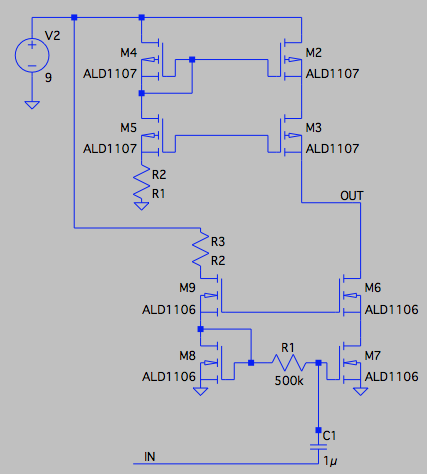
\includegraphics[width=4in,height=4in]{Cascode.png}
\caption{Cascode topology}
\end{center}
\end{figure}

After some more consideration, we decided to use multiple stages of common source topologies because they would be much easier to 
bias than cascode stage. We also decided to use MOSFETS rather than BJTs because while they had lower gain than BJTs (the $g_m$ of MOSFETS
is in the order of $10^{-3}$ compared to the BJT's $0.038$), the large gate impedance of MOS proved more attractive since we dont have to
worry much about impedance loading between stages. As for the specific MOS, we used the BS170 N-channel MOSFETs because they had high saturation
current capacity and, thus, a higher $g_m$ and gain.

Going back to the biasing of the common sources. Our first decision was to choose a desired current depending on the gain and the $V_{outBIAS}$
that we want. We will go through this calculations in a later section, but it is easy to see that both drain current and $V_{outBIAS}$ are easy
to bias. Drain current is set by using a current mirror, as shown in Figure 3.

\begin{figure}[htbp]
\begin{center}
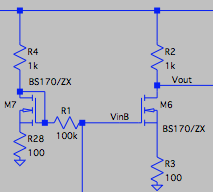
\includegraphics[width=3in,height=3in]{CurrentMirror.png}
\caption{Current Mirror Biasing a common source}
\end{center}
\end{figure}



\section{Hand Calculations and Measurements}
\subsection*{Magnitude/Phase Bode Plot}
\subsection*{Output Impedance}
\subsection*{Bias Voltages/Currents}
\subsection*{Power Consumption}

\end{document}
